\chapter{Introduction}
\thispagestyle{empty}

On 5 July, 2022, in Helsinki, Finland, the International Mathematical Union announced the names of the four mathematicians who were to be awarded the Fields Medal, the most coveted prize in the world of mathematics: Hugo Duminil-Copin, June Huh, James Maynard and Maryna Viazovska. Duminil-Copin, Huh and Maynard received this most prestigious honour for making several outstanding contributions to their specific fields of expertise---respectively, statistical physics, geometric combinatorics, and analytic number theory. Viazovska, on the other hand, received the Fields Medal for more interdisciplinary achievements. Arguably the most remarkable of these was her solution to the sphere packing problem in dimension 8 \cite{Viazovska8}. It is difficult to place her solution in a specific mathematical field: what makes it so revolutionary is that it uses insights from Fourier analysis and the theory of modular forms to construct a special function---the Magic Function---that, in combination with a previous result by Cohn and Elkies \cite{CohnElkies}, proves that the $E_8$ lattice packing is the densest possible sphere packing in $\R^8$. Very shortly afterwards, Cohn, Kumar, Miller, Radchenko and Viazovska were able to use similar ideas to prove that the Leech lattice packing is the densest possible sphere packing in $\R^{24}$ \cite{Viazovska24}.

Before Viazovska's remarkable breakthrough, the optimal sphere packing density was only known in dimensions $1$, $2$ and $3$ \cite{CohnOnViazovskaICM}. Furthermore, Thomas Hales' solution in dimension $3$ \cite{HalesKeplerInformal} was lengthy and involved extensive computer-assisted calculations; in contrast, Viazovska's proof in dimension $8$ is elegant and concise. Even before Viazovska was awarded the Fields Medal, her work received wide acclaim from eminent mathematicians across the world: Peter Sarnak described it as ``stunningly simple, as all great things are,'' and Akshay Venkatesh remarked that her Magic Function is very likely ``part of some richer story'' that connects to other areas of mathematics and physics \cite{QuantaPiece}. Viazovska's work is a truly remarkable achievement in modern mathematics, with its elegance coming from the manner in which the many pieces of the puzzle fit perfectly together. One of the goals of this project is to offer a detailed exposition of one of those pieces: the construction of the so-called `Magic Function' in dimension $8$.

\section{The Sphere Packing Problem}\label{Ch1:Sec:1_1_Sphere_Packing}

The Sphere Packing problem is a classical optimisation problem in mathematics. It goes as follows.

\begin{boxproblem}[The Sphere Packing Problem in Dimensinon $n$]\label{Ch1:Prob:SpherePacking_n}
    For some $n \in \N$, what is the densest non-overlapping arrangement of $n$-spheres of equal radius in $\R^n$?
\end{boxproblem}

Despite its straightforward formulation, \Cref{Ch1:Prob:SpherePacking_n} is notoriously difficult to solve. A key challenge in high dimensions is the fact that proceeding inductively is not always helpful: `stacking' the optimal $n$-dimensional sphere packing onto itself is not guaranteed to yield the optimal sphere packing in $n + 1$ dimensions~\cite{CohnOnViazovskaICM}. In fact, this appraoch is known to fail in dimensions as low as $10$~\cite{CohnOnViazovskaAMS}. This is not obvious, not least because the approach does, in fact, succeed in the visualisable dimensions of $1$, $2$ and $3$.

The $1$-dimensional case is uninteresting. Visually, one can easily see that the densest possible arrangement of disjoint intervals of the form $\parenth{-r, r}$ on the real line consists of intervals centred at all points $2rm$ for $m \in \Z$. Indeed, one can fix $r$ to be $\frac{1}{2}$ by rescaling the real line. The optimal packing therefore consists of open intervals of unit length centred at points on the lattice $\Z \subset \R$.

\begin{figure}[htb]
    \centering
    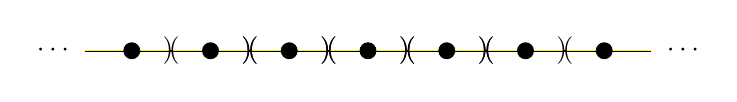
\begin{tikzpicture}
        \draw[step=1, black, thick] (-3.6, 0) -- (3.6, 0);
        \draw[yellow] (-3.6, 0) -- (-2.51, 0);
        \draw[yellow] (2.51, 0) -- (3.6, 0);
        \foreach \x in {-2, -1, 0, 1, 2} {
            \draw[yellow] (\x - 0.49, 0) -- (\x + 0.49, 0);
            \node at (\x - 0.5, 0) {$)\!($};
            \node at (\x + 0.5, 0) {$)\!($};
            \draw[fill=black] (\x, 0) circle (0.1);
        }
        \foreach \x in {-4, 4} {
            \node at (\x,0) {$\cdots$};
        }
        \draw[fill=black] (-3, 0) circle (0.1);
        \draw[fill=black] (3, 0) circle (0.1);
    \end{tikzpicture}
    \caption{The $\Z$ lattice packing in dimension $1$.}
    \label{Ch1:Fig:Z_Lattice_Packing_1D}
\end{figure}

In dimension $2$, \Cref{Ch1:Prob:SpherePacking_n}, also known as the circle packing problem, turns out to be more interesting. A reasonable strategy for finding the densest packing is to `stack' the $\Z$ lattice packing from dimension $1$ onto itself in some manner, turning these intervals into circles of the same radius. The question remains how to do this optimally.

One natural way of doing this is to stack the circles on top of themselves, turning $\Z$ into the lattice $\Z^2$, where circles are centred at points with integer coordinates: see \Cref{Ch1:Subfig:Z2_lattice_packing_2D}. Unfortunately, this packing turns out to be sub-optimal. A better candidate is the $A_2$ lattice packing: see \Cref{Ch1:Subfig:A2_lattice_packing_2D}. This packing is sometimes referred to as the \textit{honeycomb packing} due to the fact that every circle has six neighbours, whose centres form the vertices of a regular hexagon.

It is well-known that the honeycomb packing is optimal in $\R^2$. The original proof of this fact is attributed to Thue \cite{Thue}, but there are many proofs in the literature. One is outlined by Hales in \cite[p. 442]{CannonHoney}. An intuitive way of convincing oneself of Thue's theorem is that it is not possible for a circle in a given row to be in contact with more than $2$ circles in the rows above and below, meaning the $A_2$ packing cannot be improved. See \Cref{Ch1:Subfig:Kepler_Original_1}.

\begin{figure}[htb]
    \centering
    \begin{subfigure}{0.48\linewidth}
        \centering
        \begin{tikzpicture}[scale=1.25]
            \drawplane
            \foreach \x in {-2, -1, 0, 1, 2} {
                \foreach \y in {-2, -1, 0, 1, 2} {
                    \latticecircle{\x}{\y}
                }
            }
            \draw[->, color=brown, thick] (0,0) -- (1,0) node[anchor=north] {$\parenth{1, 0}$};
            \draw[->, color=brown, thick] (0,0) -- (0,1) node[anchor=east] {$\parenth{0, 1}$};
        \end{tikzpicture}
        \subcaption{The $\Z^2$ lattice packing.}
        \label{Ch1:Subfig:Z2_lattice_packing_2D}
    \end{subfigure}
    \begin{subfigure}{0.48\linewidth}
        \centering
        \begin{tikzpicture}[scale=1.25]
            \drawplane
            \clip (-2.5, -2.5) rectangle ++(5, 5);
            \foreach \x in {-4, -3, -2, -1, 0, 1, 2, 3, 4} {
                \foreach \y in {-3, -2, -1, 0, 1, 2, 3} {
                    \latticecircle{\x - \y * 0.5}{\y * 0.8660254038}
                }
            }
            \draw[->, color=brown, thick] (0,0) -- (1,0) node[anchor=north] {$\parenth{1, 0}$};
            \draw[->, color=brown, thick] (0,0) -- (-0.5,0.8660254038) node[anchor=south east] {$\parenth{-\frac{1}{2}, \frac{\sqrt{3}}{2}}$};
        \end{tikzpicture}
        \subcaption{The $A_2$ lattice packing.}
        \label{Ch1:Subfig:A2_lattice_packing_2D}
    \end{subfigure}
    \caption{Circle packings covering the square $\setst{\parenth{x, y} \subset \R^2}{-2.5 \leq x, y \leq 2.5}$.}
    \label{Ch1:Fig:Circle_Packings_2D}
\end{figure}

In dimension $3$, too, it is tempting to replicate this strategy: we can stack the $A_2$ packing on top of itself, in layers instead of rows, attempting to maximise the number of neighbours of a sphere. From trial and error, we see that a sphere cannot be in contact with more than three neighbours from the layer below. This suggests that the optimal sphere packing in dimension $3$ is given by stacking honeycomb arrangements on top of each other with spheres in each layer being nestled in the gaps between three spheres in the layer below.

\begin{wrapfigure}[28]{r}{0.27\linewidth}
    \centering
    \begin{subfigure}{\linewidth}
        \centering
        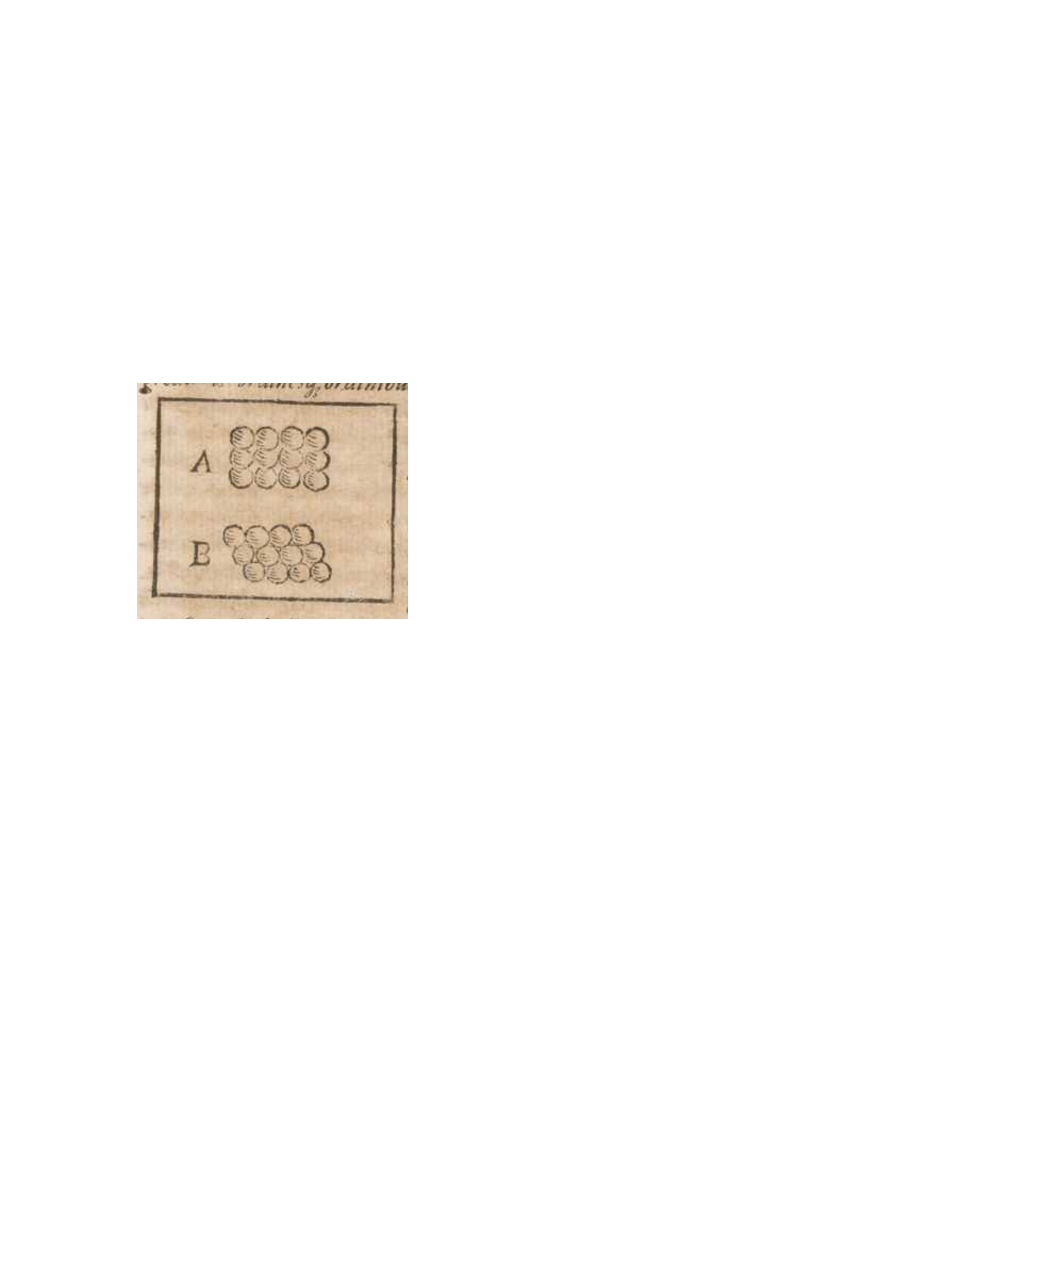
\includegraphics[width=\linewidth]{Chapters/1_Intro/Images/Kepler_1.pdf}
        \caption{}
        \label{Ch1:Subfig:Kepler_Original_1}
    \end{subfigure}
    \begin{subfigure}{\linewidth}
        \centering
        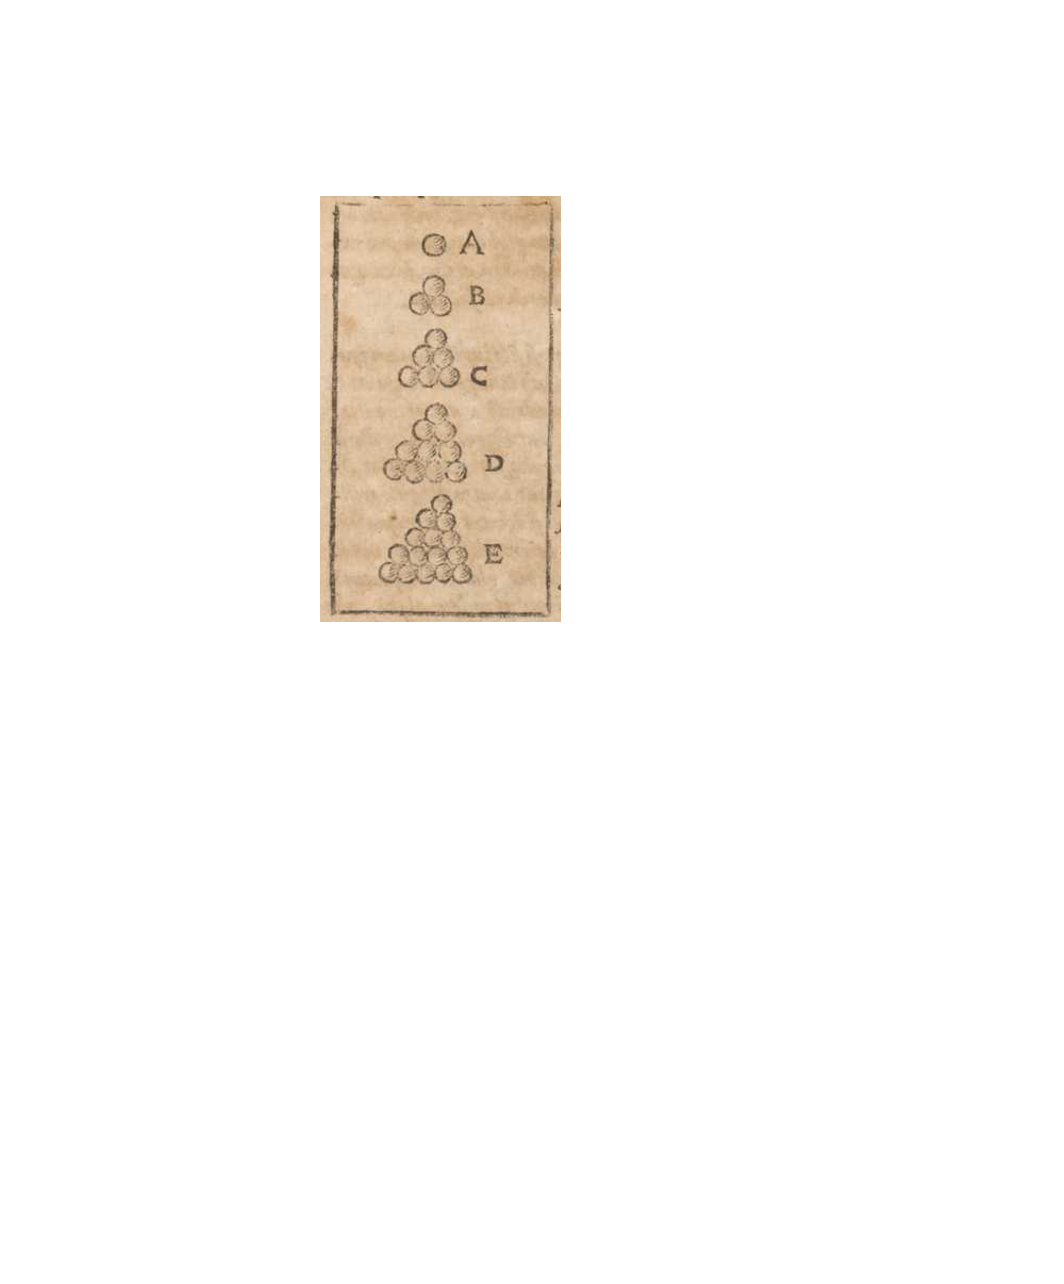
\includegraphics[width=\linewidth]{Chapters/1_Intro/Images/Kepler_2.pdf}
        \caption{}
        \label{Ch1:Subfig:Kepler_Original_2}
    \end{subfigure}
    \caption{Diagrams from an essay written by Johannes Kepler in Latin in 1611 \cite{KeplerSnowflake}.}
\end{wrapfigure}

As it turns out, unlike dimension $2$, this characterisation not describe a unique packing: spheres are simply too large! See \Cref{Ch1:Fig:2_Optimal_3D_Packings}. One can construct infinitely many locally similar, globally different sphere packings in $\R^3$, all of which are as dense as possible, by varying how successive layers are placed.

\begin{figure}[bt]
    \centering
    \begin{subfigure}{0.48\linewidth}
        \centering
        \begin{tikzpicture}[scale=1.25]
            \clip (-2.5, -2.5) rectangle ++(5, 5);
            \foreach \x in {-4, -3, -2, -1, 0, 1, 2, 3, 4} {
                \foreach \y in {-3, -2, -1, 0, 1, 2, 3} {
                    \latticecircle{\x - \y * 0.5}{\y * 0.8660254038}
                }
            }
            \foreach \x in {-3, -2, -1, 0, 1, 2} {
                \foreach \y in {-3, -2, -1, 0, 1, 2} {
                    \latticecirclegrey{\x - \y * 0.5}{\y * 0.8660254038 + 0.5773502692}
                }
            }
            \foreach \x in {-2, -1, 0, 1} {
                \foreach \y in {-2, -1, 0, 1} {
                    \latticecirclebrown{\x - \y * 0.5}{\y * 0.8660254038}
                }
            }
        \end{tikzpicture}
        \subcaption{}
        \label{Ch1:Subfig:3D_Triangular_Stacking}
    \end{subfigure}
    \begin{subfigure}{0.48\linewidth}
        \centering
        \begin{tikzpicture}[scale=1.25]
            \clip (-2.5, -2.5) rectangle ++(5, 5);
            \foreach \x in {-4, -3, -2, -1, 0, 1, 2, 3, 4} {
                \foreach \y in {-3, -2, -1, 0, 1, 2, 3} {
                    \latticecircle{\x - \y * 0.5}{\y * 0.8660254038}
                }
            }
            \foreach \x in {-2, -1, 0, 1, 2, 3} {
                \foreach \y in {-2, -1, 0, 1, 2, 3} {
                    \latticecirclegrey{\x - \y * 0.5}{\y * 0.8660254038 - 0.5773502692}
                }
            }
            \foreach \x in {-2, -1, 0, 1} {
                \foreach \y in {-2, -1, 0, 1} {
                    \latticecirclebrown{\x - \y * 0.5}{\y * 0.8660254038 + 0.5773502692}
                }
            }
        \end{tikzpicture}
        \subcaption{}
        \label{Ch1:Subfig:3D_Hexagonal_Stacking}
    \end{subfigure}
    \caption{Two different ways of stacking the honeycomb packing on itself.}
    \label{Ch1:Fig:2_Optimal_3D_Packings}
\end{figure}

This observation is not novel. In a 1611 essay whose title has been translated from Latin as \textit{The Six-Cornered Snowflake} \cite{KeplerSnowflake}, Johannes Kepler asserted that spheres cannot be more tightly packed together than they are in a tetrahedral arrangement: see \Cref{Ch1:Subfig:Kepler_Original_2}. This result became known as the Kepler Conjecture, and it went unproven for over three centuries, until 2005 that a paper proving it, written by Thomas Hales, was published \cite{HalesKeplerInformal}.

The complexity of the sphere packing problem in dimension $3$ is illustrated not only by the time elapsed between Kepler's original assertion and a proof being published but also by the length of Hales's paper. Indeed, in an expository account of his proof published in 2000, five years before the publication of the full paper in the Annals, Hales recounted how a jury of twelve referees, despite having been in deliberation for over a year, had yet to make a ``thorough, independent check of the computer code'' he had written to perform the elaborate calculations on which ``every aspect of [his proof] is based'' \cite{CannonHoney}. In January 2003, at the Joint Math Meetings in Baltimore, USA, Hales announced that he intended to formally verify his proof \cite{HalesKeplerFormal}, in what he termed the Flyspeck project. The paper authored by Hales and his collaborators on their successful formalisation of his argument was only published in 2017. Therefore, not only did the Kepler Conjecture take close to 400 years to solve, but it took nearly two decades to eliminate any doubt as to the correctness of the solution. This project aims to formalise a result of a similar flavour in a significantly shorter timeframe.
\section{The Formalisation Movement}

While Hales announced his intent to formally verify his proof of the Kepler Conjecture in 2003, it was not till 2006, after Hales's solution appeared in the \textit{Annals}, that a formal description of Hales's formalisation project was published. Of his motivations, Hales wrote:
\begin{quote}
    \textit{In response to the lingering doubt about the correctness of the proof, at the beginning of 2003, I launched the \emph{Flyspeck} project, whose aim is a complete formal verification of the Kepler Conjecture. In truth, my motivations for the project are far more complex than a simple hope of removing residual doubt from the minds of few referees. Indeed, I see formal methods as fundamental to the long-term growth of mathematics.}~\cite{FlyspeckAnnouncement}
\end{quote}
Formal theorem proving was not unheard of in 2006. Interactive theorem provers, such as Coq and PRL, have existed since the 1980s. However, it was a relatively young field, and the amount of mathematics that had been formalised was limited. Hales's project was immensely ambitious, and the fact that it succeeded, despite taking over a decade, is impressive.

There is something prophetic about Hales's ``far more complex'' motivations for launching the Flyspeck project. The field of formal theorem proving has grown rapidly in the last decade, and interactive theorem provers like Lean are slowly making their way into mainstream mathematics. An excellent example of this is the formal verification of Gowers, Green, Manners and Tao's proof of Marton's Conjecture~\cite{PFRPublished}, which was formally verified in Lean in just three weeks. In particular, their proof was formally verified \textit{before} their paper was submitted for publication. The paper appeared in the \textit{Annals} in March 2025.

While this project has its similarities to Flyspeck, the objectives are slightly different. There is significant consensus in the mathematical community as to the correctness of Viazovska's result, and suspicions that $E_8$ is optimal in $\R^8$ existed long before her paper was published. The project is instead a challenge to the formalisation community---an attempt to push the capabilities of modern interactive theorem proving by formalising a Fields Medal-winning result mere years after its publication and sooner still after it was given this most prestigious recognition. While cutting-edge mathematics has been formalised before \cite{liquidtensor}, formalising a result of the prestige, nuance, and incredible beauty of Viazovska's would be a landmark achievement of modern formalisation.
\section{The Scope of this Project}

% Ask how to word this... is "I" ok??

In November 2023, I had the privilege of meeting Maryna Viazovska while pursuing an exchange programme at the Swiss Federal Institute of Technology, Lausanne, where she is based. We began discussing formalising her solution to the sphere packing problem in $8$ dimensions, and soon initiated a collaboration with Christopher Birkbeck, Seewoo Lee, and Gareth Ma, with invaluable assistance from Kevin Buzzard, Utensil Song, and Patrick Massot. On 31 May 2024, Viazovska formally announced at the ICMS workshop \textit{Formalisation of Mathematics: Workshop for Women and Mathematicians of Minority Gender} that we would be attempting to formalise her groundbreaking paper.

Viazovska's original paper~\cite{Viazovska8} is divided into five sections. The first section introduces sphere packings and develops basic theory; the second discusses the Cohn-Elkies linear programming bounds~\cite[Theorem 3.1]{CohnElkies}; the third offers some background on the theory of modular forms; the fourth constructs two radial, Schwartz Fourier eigenfunctions with double zeroes at almost all points on the $E_8$ lattice; and finally, the fifth uses these eigenfunctions to construct the ``Magic Function'', a Schwartz function that satisfies the conditions of Cohn and Elkies's theorem to give an upper bound for all sphere packings in $\R^8$ that is equal to the density of the $E_8$ packing. The first two sections were formalised collaboratively in July and August 2024, and the third section is actively being worked on by Birkbeck and Lee. This project focuses on formalising the fourth and fifth sections of Viazovska's paper. The code written for this section is primarily my own, and I have credited the contributions of others where appropriate.

The primary objective of this thesis is to offer a mathematical exposition of the fourth and fifth sections of Viazovska's original paper and to provide an account of the formalisation process. \todo{Say where we are with the formalisation before submitting.}

\begin{comment}
    Given the limitations of the M4R assessed project paradigm, I decided, at the very beginning, to use the first three sections of Viazovska's paper as a black box in order to reduce the number-theoretic burden on what already stood ahead of me as a daunting formalisation task. In particular, I chose not to make this M4R a number theory project with an element of formalisation but a formalisation project involving ideas from number theory and complex analysis. This conscious but deliberate decision illustrates one of the many advantages of formal theorem proving: modularity with assurances. That is, one need not understand the entirety of a project to contribute to it: one simply needs to understand the parts one is formalising and how to use other ideas and results to one's end. In particular, the fact that the results one is using are formalised provides one with the assurance (that would otherwise only come with expertise) that those results are, indeed, correct. By bearing in mind the subtle yet immensely important fact that this project, at its core, is not a number theory project but a formalisation project, the reader will better understand the expository choices made by the author over the course of this report. There will be less emphasis on the motivations for constructing Viazovska's magic function in this manner (for there exist numerous excellent expository articles that explain this in detail \cite{a few things}) and more emphasis on the formalisation process, with reflections on the successes and failures of the formalisation strategies employed. We underscore insights gleaned from doing this that were not evident in the paper, one one occasion even identifying a small (but negligible) error that was published in the Annals. 
\end{comment}